\documentclass[12pt,a4paper]{article}
\usepackage[utf8]{inputenc}
\usepackage[T1]{fontenc}
\usepackage[ngerman]{babel}
\usepackage{amsmath}
\usepackage{amsfonts}
\usepackage{amssymb}
\usepackage{graphicx}
\usepackage{packets}
\author{Lars Döpper}
\date{\today}
\title{441 Computerphysik - Hausaufgabe 1}

\begin{document}
	\maketitle
\section{Aufgabe 1 - Elektrostatisches Potential}
\subsection{Potential der Ladungsverteilung}
Zunächst möchte wir die Ladungsverteilung $\rho(x,y,z)$ normieren. Dafür berechnen wir:
\begin{align}
	\int_{-\infty}^{\infty}\rho(x,y,z)d^3x &= Q
\end{align}
Wir erhalten durch Integrieren über die Delta-Distributionen:
\begin{align}
	\alpha\frac{Q}{a}\int_{-\infty}^{\infty}\exp\left(-\frac{x^2}{a^2}\right)dx &= Q
\end{align}
Und nach der Auswertung des Gauß-Integrals erhalten wir schließlich:
\begin{align}
	\alpha*Q*\sqrt{\pi} &= Q
\end{align}
Damit folgt, dass $\alpha = \frac{1}{\sqrt{\pi}}$. Dies setzen wir später als eine Konstante im Programmcode fest. Des weiteren wissen wir auch, dass für das Elektrostatische Potential gilt:
\begin{align}
	V(x,y,z) &= \frac{1}{4\pi\epsilon_0}\int_{-\infty}^{\infty}\frac{\rho(x',y',z')}{|\vec{x}-\vec{x'}|}d^3x' \\
	&= \frac{\alpha Q}{4\pi\epsilon_0a}\int_{-\infty}^{\infty}\dfrac{\exp(-\frac{x'^2}{a^2})}{|(x-x')^2 + y^2 +z^2|}d^3x' \\
	&= \frac{\alpha Q}{4\pi\epsilon_0a}\int_{-\infty}^{\infty}\dfrac{\exp(\frac{-x'^2}{a^2})}{|x'^2 + z^2|}d^3x'
\end{align}
Somit hängt der Wert unsere Potentials in z-Richtung nur noch von z selber und einem Integral ab, welches wir im folgenden numerisch lösen werden.

\subsection{Integration des Romberg-Verfahrens}
Als nächstes integrieren wir das Romberg-Verfahren, um das uneigentliche Integral zu berechnen. Da der Integrand für große x sehr schnell gegen 0 abfällt, müssen wir das Integral nur auf einem Teilbereich berechnen und nicht auf ganz $ \mathds{R} $. Schon für $x > 20$ überschreitet der Wert des Integranden den Maximalwert des Datentyps \verb|double|, deswegen verwenden wir dies im Folgenden als symmetrische Grenzen des Integrals. Der Rest der Implementierung lässt sich in den Dateien \verb|hausaufgabe1.c| und \verb|numerik_own.c| finden.

\subsection{Die charakteristische Breite a}
Nachdem wir in der letzten Aufgabe das Romberg-Verfahren implementiert haben, können wir dieses nun nutzen, um uns die Werte des Potentials $V(z)$ auf dem Intervall $[0,5]$ anzeigen zu lassen. Dabei variieren wir die Werte der charakteristischen Breite $a$ zwischen $4$ und $0.001$ um den Grenzfall $\lim a \rightarrow 0$ zu simulieren. Die dazugehörigen Graphen sehen wir in Abbildung \ref{abb_1}.
\begin{figure}[htbp]
	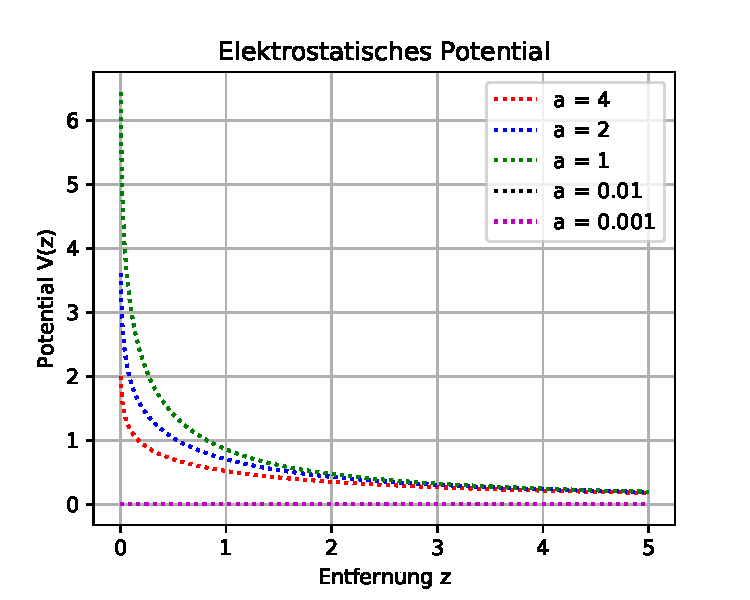
\includegraphics[width=0.8\textwidth]{aufgabe1.pdf}
	\caption{Elektrostatisches Potential verschiedener charakteristischer Breiten}\label{abb_1}
	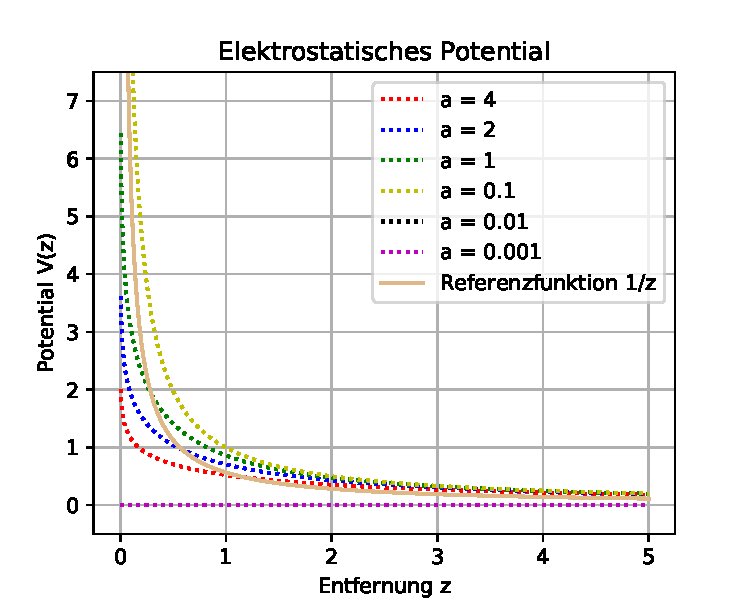
\includegraphics[width=0.8\textwidth]{aufgabe1_referenzpot.pdf}
	\caption{Potential mit Vergleichsfunktion}\label{abb_2}
\end{figure}
Wir sehen, dass sich das Potential mit niedrigerer charakteristischen Breite $a$ immer mehr an eine $\frac{1}{z}$ Funktion annähert, wie man es für eine Punktladung erwarten würde. Allerdings wird das Integral ab einer gewissen Breite nur noch zu 0 ausgewertet, da der Exponent der Exponentialfunktion mit fallendem $a$ immer stärker zunimmt und irgendwann die Maximalgröße des Datentyps überschritten wird. Dies geschieht bei den ausgewählten Breiten zwischen $a_4 = 0.1$ und $a_5=0.01$. Damit entspricht zwar die allgemeine Entwicklung des Potentials den Erwartungen, allerdings unterschreiten wir ab einem gewissen Punkt die Genauigkeit des Computers und das Potential wird nur noch zu $V(z) = 0$ ausgewertet, was nicht den Erwartungen eines Punktladungspotentials entspricht.

\section{Aufgabe 2 -Elektrisches Feld}
\subsection{Berechnung des Elektrischen Feldes}
In dieser Aufgabe berechnen wir aus dem Potential aus Aufgabe 1 das Elektrische Feld der Ladungsverteilung $\rho(x',y',z')$. Für das Elektrische Feld eines Potentials in z-Richtung gilt:
\begin{equation}
	\vec{E(z)} = -\vec{\nabla_z}V(x,y,z) = -\frac{\partial V}{\partial z}(x,y,z)
\end{equation}
Wir können diese Ableitung numerisch durch den symmetrischen Differenzenquotienten annähern. Wir erhalten damit das folgende Elektrische Feld: \ref{f:e_field}.
\begin{figure}[htbp]
	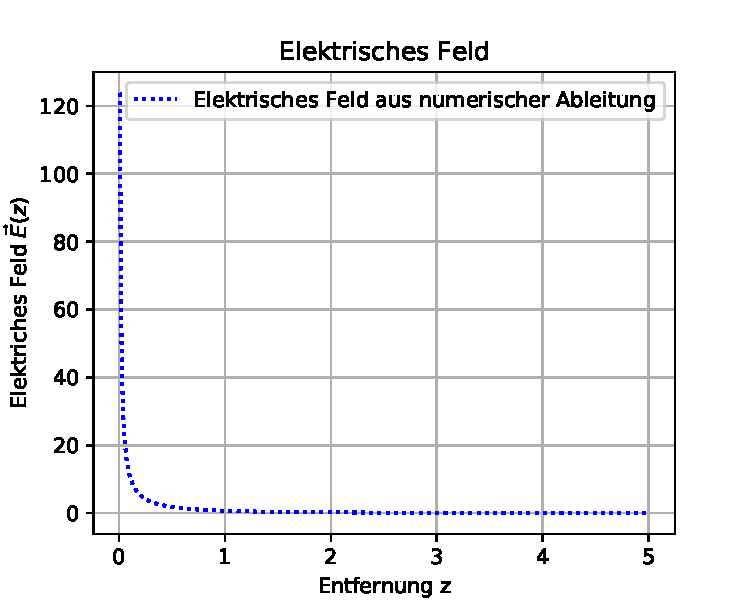
\includegraphics[width=0.8\textwidth]{aufgabe2_1.pdf}
	\caption{Elektrisches Feld der Ladungsverteilung}
	\label{f:e_field}
\end{figure}
\subsection{Überprüfung der numerischen Ableitung}
Wir können die numerische Ableitung nun auch analytisch überprüfen. Für das Elektrische Feld gilt:
\begin{align*}
	\vec{E}(z) &= -\frac{\partial V}{\partial z}(z) \\
	&= -\frac{\partial}{\partial z}\frac{\alpha Q}{4\pi \epsilon_0 a}\int_{-\infty}^{\infty}\frac{\exp(-x^2/a^2)}{\sqrt{x^2+z^2}}dx \\
	&= \frac{\alpha Q}{4\pi \epsilon_0 a}\int_{-\infty}^{\infty}\frac{\partial}{\partial z} \frac{\exp(-x^2/a^2)}{\sqrt{x^2+z^2}}dx \\
	&= \frac{\alpha Q}{4\pi \epsilon_0 a}z\int_{-\infty}^{\infty} \frac{\exp(-x^2/a^2)}{ (x^2+z^2)^{3/2}} dx
\end{align*}
Wir können uns also eine neue Funktion für das Elektrische Feld definieren, die auch wieder die Romberg-Integration nutzt, um den Wert des Elektrischen Feldes zu berechnen.
Wie wir in Abbildung \ref{f:e_field_2} sehen können, sind die beiden Graphen deckungsgleich, somit stimmen die Ergebnisse überein und dieser Verlauf spiegelt das Elektrische Feld in z-Richtung wieder.
\begin{figure}[htbp]
	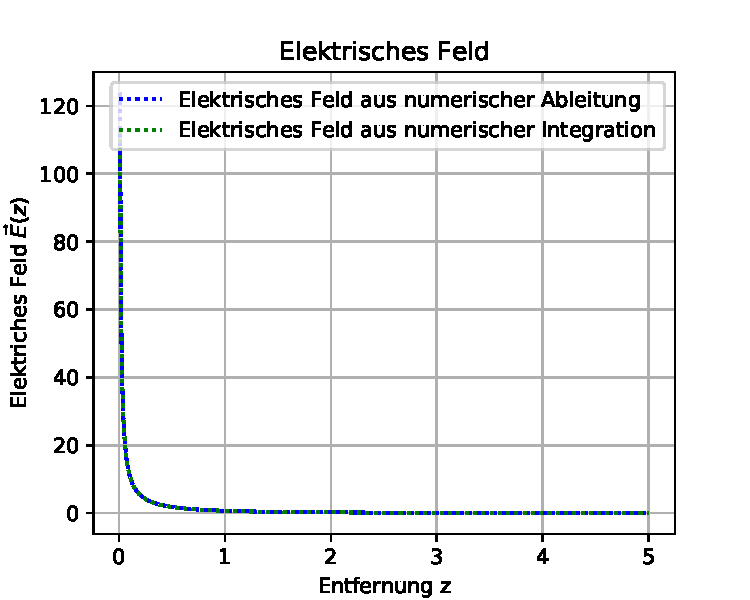
\includegraphics[width=0.8\textwidth]{aufgabe2_2.pdf}
	\caption{Vergleich von numerischer Ableitung und Integration}
	\label{f:e_field_2}
\end{figure}
\section{Aufgabe 3 - Gleichgewichtspunkt}
\subsection{Implementierung}
In dieser Aufgabe befassen wir uns mit einer leicht veränderten Ladungsverteilung. So sind dieses Mal zwei Ladungen auf zwei Drähten um unsere Probeladung verteilt. Nach dem Superpositionsprinzip gilt damit für das Elektrostatische Potential an der Stelle z.
\begin{equation}
	V_G(z) = V_1(z) + V_2(d-z)
\end{equation}
Somit lässt sich die Berechnung aufteilen in zwei Potentiale, die wir genau so wie in Aufgabe 1 berechnen können. Das gleiche gilt für das Elektrische Feld. Der abschließende Term für das Elektrische Feld lautet:
\begin{equation}
	E(z) = \frac{\alpha}{4\pi\epsilon_0}\left[\frac{Q_1}{a_1}z\int_{-\infty}^{\infty}\frac{\exp(-x^2/a_1^2)}{(x^2 + z^2)^{3/2}}
	-\frac{Q_2}{a_2}(d-z)\int_{-\infty}^{\infty}\frac{\exp(-x^2/a_2^2)}{(x^2 + (d-z)^2)^{3/2}}\right]
\end{equation}
Mit diesem Term für das Elektrische Feld erhalten wir den Graphen in Abbildung \ref{f:e_field_3}.
\begin{figure}[htbp]
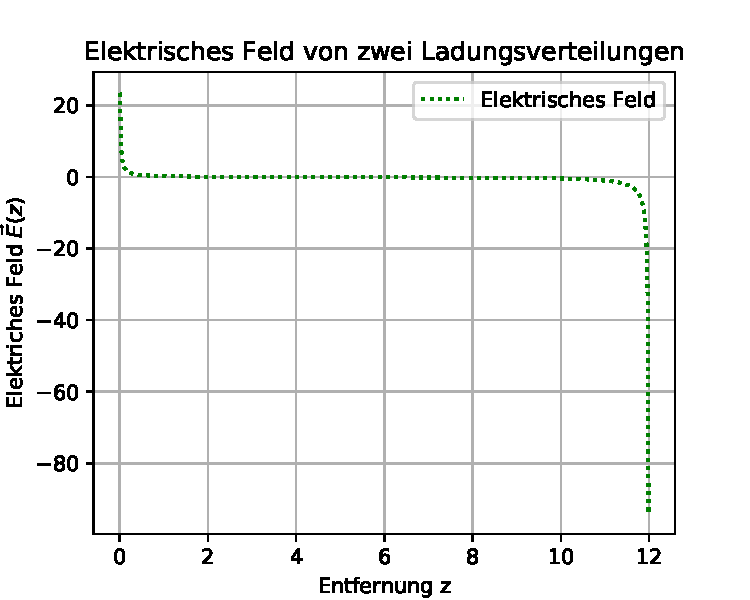
\includegraphics[width=0.8\textwidth]{aufgabe3_1.pdf}
\caption[Elektrisches Feld]{Elektrisches Feld der beiden Ladungsverteilungen}
\label{f:e_field_3}
\end{figure}
\subsection{Bestimmung des Gleichgewichtspunktes}
Wir haben also nun eine Funktion für das Elektrische Feld dieser Ladungsverteilung. Für den Gleichgewichtspunkt muss dann gelten:
\begin{equation*}
	\vec{E}(z) = 0
\end{equation*}
Um diesen Punkt zu bestimmen, können wir das Sekanten-Verfahren auf diese Funktion anwenden und so die Nullstelle bestimmen. Dies führen wir für verschieden Werte von $a_2$ durch, wobei gelten muss: $a_1/10 \leq a_2 \leq a_1$. Wir können die so gefundenen Werte der Nullstellen gegen $a_2$ auftragen und so einen Zusammenhang erkennen. Diesen Graph kann man in Abbildung \ref{f:nullstellen} sehen. Der Graph lässt auf einen exponentiellen Zusammenhang zwischen Breite $a_2$ und der Lage des Gleichgewichtspunktes schließen, aber ohne eine genauere Untersuchung lässt sich nicht mehr als das sagen.
\begin{figure}[htbp]
	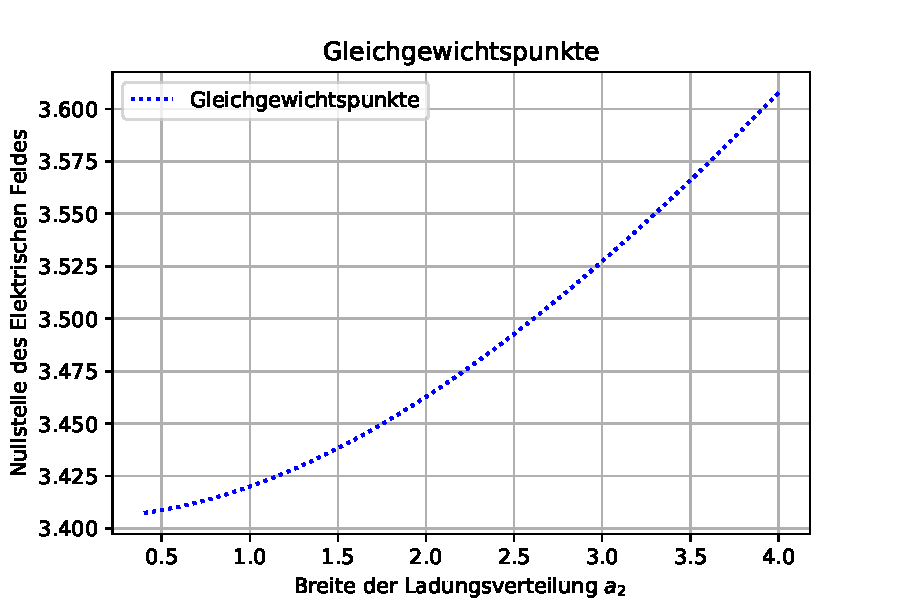
\includegraphics[width=0.8\textwidth]{Nullstellen.pdf}
	\caption{Gleichgewichtspunkt in Abhängigkeit von $a_2$}
	\label{f:nullstellen}
\end{figure}
\newpage
\listoffigures
\end{document}